\documentclass[lettersize,journal]{IEEEtran}
\usepackage{amsmath,amsfonts}
\usepackage{algorithmic}
\bibliographystyle{IEEEtran}
\usepackage{algorithm}
\usepackage{array}
\usepackage[caption=false,font=normalsize,labelfont=sf,textfont=sf]{subfig}
\usepackage{textcomp}
\usepackage{stfloats}
\usepackage{url}
\usepackage{verbatim}
\usepackage{graphicx}
\usepackage{cite}
\usepackage{tikz}
\usetikzlibrary{shapes.geometric, arrows, positioning, fit, calc, backgrounds}
\hyphenation{op-tical net-works semi-conduc-tor IEEE-Xplore}

\begin{document}

\title{Multi-Agent Debate Framework for Comprehensive UAV Swarm Performance Evaluation}

\author{Shuai Hao, Haibin Duan and Chen Wei

\thanks{This paper was produced by the IEEE Publication Technology Group. They are in Piscataway, NJ.}% <-this % stops a space
\thanks{Manuscript received April 19, 2021; revised August 16, 2021.}}


\maketitle
%------------------------------------------------------
\begin{abstract}
This paper presents a novel multi-agent debate system for comprehensive UAV swarm performance evaluation. Unlike traditional single-perspective assessment methods, our approach leverages multiple specialized AI agents representing different domains of expertise to engage in structured evaluation dialogues, ensuring holistic coverage of critical performance dimensions. The proposed methodology integrates six innovative mechanisms: (1) hierarchical debate structure that dynamically routes issues by complexity to optimize computational efficiency, (2) adversarial-collaborative protocol with rotating red-blue teams to eliminate confirmation bias and echo chamber effects, (3) dynamic role rotation across debate rounds to prevent perspective lock-in, (4) evidence chain traceability ensuring all claims are backed by verifiable trajectory data, (5) multi-dimensional consensus modeling to quantify agreement patterns and identify disagreement types, and (6) meta-cognitive quality monitoring with real-time interventions to maintain debate rigor. We demonstrate the proposed methodology's effectiveness through comprehensive evaluation of real UAV swarm trajectory data, showing that the multi-agent debate approach produces more thorough, balanced, and actionable assessments compared to conventional single-metric or fixed-weight evaluation methods. Our contributions provide a principled methodology for UAV swarm evaluation that is adaptable to diverse mission types and operational environments.

\end{abstract}

\begin{IEEEkeywords}
UAV swarm evaluation, multi-agent debate, collaborative AI, adversarial reasoning, consensus modeling, evidence-based assessment, structured argumentation.
\end{IEEEkeywords}
%--------------------------------------------------------

\section{Introduction}
\IEEEPARstart{T} he proliferation of Unmanned Aerial Vehicle (UAV) swarms in civilian and military applications has created an urgent need for comprehensive, objective, and multi-dimensional performance evaluation approaches. UAV swarms present unique challenges in assessment due to their complex interdependencies, real-time coordination requirements, and multi-faceted performance criteria spanning flight control, inter-vehicle communication, formation stability, and safety protocols. Traditional single-perspective evaluation methods often fail to capture the nuanced interactions and trade-offs inherent in swarm systems, leading to incomplete or biased assessments that may overlook critical performance aspects.

\subsection{The Critical Problem: Three Fundamental Bottlenecks}

Despite significant advancements in UAV technology, the evaluation methodology lags behind, facing three critical bottlenecks that directly impact safety and reliability:

\noindent\textbf{(1) The "Black-Box" Dilemma:} Modern swarm algorithms are inherently opaque, making it extremely difficult to understand \textit{why} failures occur. Traditional metrics like RMSE (Root Mean Square Error) can tell us \textit{that} a performance deviation exists, but fail to explain the root causes. For instance, a high RMSE value might indicate poor trajectory tracking, but cannot distinguish whether the problem stems from sensor noise, control system instability, or communication delays. This lack of interpretability makes it impossible to provide actionable feedback for system improvement, and hinders debugging of critical failures in safety-critical scenarios.

\noindent\textbf{(2) The Subjectivity vs. Scalability Gap:} Human expert evaluation provides comprehensive, contextual assessment but is unscalable—a team of three experts requires 15-30 minutes per mission, making exhaustive testing of thousands of flights impractical. Conversely, automated metrics can scale but lack contextual understanding. For example, an automated system might flag a formation deviation of 1.2 meters as a failure, but fail to recognize that this deviation occurred during a successful collision avoidance maneuver where maintaining formation was intentionally sacrificed. Without contextual reasoning, automated evaluation produces either false positives (alerting on acceptable behaviors) or false negatives (missing real issues).

\noindent\textbf{(3) Lack of Adversarial Validation:} Most evaluation approaches operate under a \textit{verification} mindset—checking that the system meets specified requirements—rather than actively hunting for edge cases and potential failure modes. This leads to "Toxic Positivity," where high average scores mask critical risks. For instance, a swarm might achieve 95\% formation stability overall, but in rare edge cases (e.g., during GPS multipath interference or sudden obstacle avoidance), the formation could completely collapse, causing catastrophic failure. Without adversarial validation that actively seeks out and tests these edge cases, such latent risks remain undetected until they occur in real operations.

\subsection{Current Approaches and Their Limitations}

Current research in UAV swarm evaluation generally falls into two categories, both inadequate for addressing the bottlenecks above:

\textit{Metric-Aggregation Methods} compute weighted sums of physical parameters \cite{ali2020path}, such as trajectory tracking error, formation stability, and communication quality. While these methods are objective and scalable, they suffer from rigidity—fixed weights cannot adapt to mission-specific nuances. More critically, they cannot provide explanatory insights or detect edge cases, failing to address all three bottlenecks: they remain opaque (no root cause analysis), lack contextual understanding (rigid weights), and lack adversarial validation (passive verification only).

\textit{Single-Agent LLM Assessment} uses Large Language Models for log analysis \cite{xi2023rise}. While LLMs can provide natural language explanations, single-agent setups often suffer from hallucinations (fabricating events not present in data) and lack the rigor required for safety-critical tasks. More importantly, a single LLM acts as a "yes-man" that validates implicit biases rather than providing independent assessment. If the model is trained on data primarily showing successful flights, it may be overly optimistic and fail to detect rare but critical failure patterns—exacerbating the Toxic Positivity problem.

\subsection{Related Work and Context}

Beyond UAV-specific evaluation, two broader research areas are relevant to our approach: multi-agent cognitive architectures and explainable AI (XAI).

\textit{Multi-Agent Cognitive Architectures:} Multi-LLM debate aims to improve answer correctness through iterative argumentative exchange \cite{irving2018ai, du2023improving}. While effective for general QA tasks, existing approaches suffer from "echo chamber" effects when agents share correlated biases \cite{liang2023encouraging}. This limitation is particularly problematic for safety-critical domains like UAV swarm evaluation, where diverse perspectives are essential. Recent work has explored adversarial role assignment to mitigate this issue, but these approaches lack domain-specific grounding and evidence-based validation.

\textit{Explainable AI (XAI):} XAI research has explored saliency maps and attention mechanisms for visualizing decisions \cite{wei2022chain, wang2022self}. While these methods provide insights into model behavior, they are often too technical for operators and lack the contextual reasoning needed for complex system evaluation. Natural language explanations offer better accessibility, but single-agent explanations lack the rigor of stress-testing by opposing perspectives.

\textit{UAV Swarm Evaluation Paradigms:} Traditional UAV evaluation focuses on individual agent metrics like trajectory tracking error \cite{ali2020path, NASA} or extended collective metrics like formation stability and communication quality \cite{schranz2020swarm}. Recent advances in Deep Reinforcement Learning and evolutionary algorithms have improved autonomous control \cite{LI20221697, machines10111033, ZHANGJiandong, chaijiajun, leiyangqi, wanying, wanyingzdhxb, nankai, hagongda, hanguo}, but evaluation still relies on aggregate reward functions \cite{drone_racing} or simple success metrics, lacking the adversarial validation and explanatory depth required for safety-critical assessment.

Our work bridges the gap between these research areas by incorporating trajectory-specific evidence chains, safety-critical monitoring, and adversarial validation mechanisms tailored to cyber-physical systems. We address the echo chamber problem through explicit adversarial role assignment, and we enhance explainability by grounding all claims in verifiable trajectory data.

\subsection{Our Method: Multi-Agent Debate for UAV Swarm Evaluation}

To address these fundamental bottlenecks, we propose a novel method that transforms UAV swarm evaluation from a passive verification task into an active, adversarial, and comprehensive assessment process. The core idea is to simulate an expert panel debate through structured interactions between multiple specialized AI agents, combining the scalability and objectivity of automated systems with the contextual understanding and edge-case detection capabilities of human experts.

\textbf{Method Overview:} The evaluation proceeds through a three-stage process. First, raw UAV trajectory data is converted into a structured Domain Specific Language (DSL) that preserves critical kinematic information while compressing data by approximately 85\%. Second, multiple specialized agents engage in iterative debate rounds, where each agent generates structured assessments with explicit evidence citations, critiques other agents' viewpoints, and refines their own judgments based on peer feedback. Third, a multi-dimensional consensus mechanism aggregates agent opinions across four dimensions (score, semantic, priority, and concern) to produce the final evaluation report.

\textbf{Addressing the Black-Box Dilemma via Evidence-Based Reasoning:} To overcome the opacity of traditional metrics, our method enforces \textbf{Evidence Chain Traceability}. Every claim made by an agent must be backed by verifiable citations to specific trajectory segments using standardized DSL tokens (e.g., "Risk at SEG[4]: t=20-25, proximity violation of 1.2m"). The validation process operates as follows: (1) Each agent's response is parsed to extract claims and their supporting evidence; (2) The DSL citations are verified against the actual trajectory data; (3) Unsupported claims are flagged and rejected. This mechanism ensures that all explanations are grounded in concrete data, making root causes explicit and enabling targeted debugging. For example, instead of reporting "poor trajectory tracking," the method would specify "SEG[7]: t=35-40, heading deviation of 15deg coincides with GPS dropout at t=37," directly identifying the sensor failure as the root cause.

\textbf{Bridging the Subjectivity vs. Scalability Gap via Specialized Agent Roles:} Our method leverages three specialized agents, each with distinct cognitive biases designed to simulate different expert perspectives:

\begin{itemize}
    \item \textbf{Flight Control Specialist (FCS):} Operates with a precision bias, prioritizing quantitative metrics (RMSE, variance) and penalizing deviations $>5\%$ from nominal trajectories. Focuses on physical feasibility of maneuvers and energy efficiency.

    \item \textbf{Swarm Coordination Expert (SCE):} Operates with a cohesion bias, evaluating the swarm as a collective entity. Uses a global view that suppresses individual outlier data in favor of group statistics, penalizing formation breaks even if individual paths are safe.

    \item \textbf{Safety Assessment Expert (SAE):} Operates with a pessimistic bias under a "zero-trust" model. Flags any state vector approaching within 10\% of safety envelope boundaries as critical risk, prioritizing false positives over false negatives.
\end{itemize}

Through structured debate, these agents combine their specialized knowledge to achieve context-aware evaluation. For instance, when analyzing a formation deviation that occurred during collision avoidance, SCE might initially flag it as a failure, but FCS would provide context that the deviation was necessary for safety, and SAE would verify that the new configuration maintained safe distances. The debate process automatically resolves such trade-offs, reasoning about whether "formation deviation acceptable given successful collision avoidance"—a capability that automated fixed-weight metrics cannot achieve. The entire process completes in an average of 12.3 seconds per mission, enabling evaluation of thousands of flights.

\textbf{Enabling Adversarial Validation via Red-Blue Team Protocol:} To actively hunt for edge cases and eliminate confirmation bias, our method implements a dynamic adversarial protocol. In each debate round, agents are assigned to either the Red team (adversarial) or Blue team (collaborative), with assignments rotating across rounds using a round-robin scheme.

\textbf{Red Team Instructions:} Agents in the adversarial role are explicitly prompted to: (1) actively search for anomalies and potential risks in the data; (2) challenge overly optimistic scores with concrete counter-examples; (3) identify boundary cases where the system approaches but does not violate safety thresholds; (4) question assumptions made by other agents; and (5) flag patterns that might indicate rare but critical failure modes.

\textbf{Blue Team Instructions:} Agents in the collaborative role are prompted to: (1) provide objective professional assessment based on domain expertise; (2) acknowledge valid criticisms from the Red team with data-backed evidence; (3) refute unreasonable challenges by citing specific trajectory segments; and (4) maintain a constructive stance focused on improving system design.

The adversarial framing ensures comprehensive coverage of edge cases. For example, a mission might achieve high average formation stability (95\%) but contain a rare 2-second window where GPS multipath interference caused temporary loss of coordination. A single-metric approach would miss this critical risk. In our method, the Red team SAE, operating with its pessimistic bias and adversarial instructions, would specifically search for and identify this anomaly, flagging it as a safety concern even though the overall metrics look good. Empirical results show that this adversarial method achieves 96\% recall in safety issue detection (24 out of 25 confirmed violations), compared to only 71\% for single-agent LLM baseline.

\subsection{Our Contributions}

This paper makes the following specific contributions:

\textbf{(1) Six Novel Mechanisms:} We introduce a comprehensive methodology integrating: (a) \textbf{Hierarchical debate structure} that dynamically routes issues by complexity to optimize computational efficiency (59\% token reduction); (b) \textbf{Adversarial-collaborative protocol} with rotating red-blue teams to eliminate confirmation bias; (c) \textbf{Dynamic role rotation} across debate rounds to prevent perspective lock-in; (d) \textbf{Evidence chain traceability} ensuring all claims are backed by verifiable trajectory data; (e) \textbf{Multi-dimensional consensus modeling} to quantify agreement patterns and identify disagreement types; and (f) \textbf{Meta-cognitive quality monitoring} with real-time interventions to maintain debate rigor.

\textbf{(2) Empirical Validation:} We demonstrate effectiveness through comprehensive evaluation of 50 real UAV swarm missions, achieving 91\% agreement with human expert consensus (Cohen's $\kappa$ = 0.84) compared to 74\% for single-agent LLM. Our proposed system achieves 96\% recall in safety issue detection with zero hallucination rate, versus 71\% recall and 14\% hallucination rate for baselines.

\textbf{(3) Scalable Deployment:} The proposed system evaluates missions in 12.3 seconds at \$0.13 per mission—two orders of magnitude cheaper than human expert review (\$15-30) while maintaining near-human accuracy, enabling exhaustive evaluation of thousands of flights.

The system's modular design allows adaptation to diverse UAV platforms and mission types, making it a versatile tool for the rapidly evolving UAV industry.





\section{Methodology}

\subsection{Trajectory Abstraction and Evidence Representation}

To bridge the gap between continuous numerical trajectory data and linguistic reasoning capabilities of LLMs, we implement a specialized Trajectory Domain Specific Language (DSL). This module compresses raw flight data into a structured textual representation that preserves critical semantic information while fitting within the LLM's context window.

The abstraction process involves three steps:
1) Segmentation: The trajectory is divided into logical segments based on kinematic properties (e.g., straight flight, turning, climbing) using a sliding window approach with change-point detection on heading and speed.
2) Event Extraction: Critical flight events are identified, including sharp turns ($>30^\circ$), rapid altitude changes ($>3 \text{m/s}$), and proximity alerts.
3) DSL Generation:** The segmented data is formatted into a compact textual block using standardized tokens: \texttt{SEG} (segment details), \texttt{EVENT} (critical anomalies), \texttt{ATTN} (attention-worthy regions), \texttt{WAYPTS} (waypoint deviations), and \texttt{SCORES} (metric summaries).

For example, a turn maneuver is represented as:
\texttt{SEG[2]: t=15-25, dir=NE->E, v=12.5$\pm$0.5, turn=high}
\texttt{EVENT: t=20, sharp\_turn=45deg}

This structured DSL allows agents to cite specific "SEG" or "EVENT" identifiers as verifiable evidence in their arguments, enabling the Evidence Chain Traceability mechanism described in Section III-D.

Table \ref{tab:dsl_vocab} summarizes the key vocabulary used in our Trajectory DSL. By discretizing continuous signals into these semantic tokens, we reduce the token usage by approximately 85\% compared to raw numerical arrays, while retaining the causal information necessary for logical deduction.

\begin{table}[h]
\caption{Trajectory DSL Vocabulary and Semantics}
\label{tab:dsl_vocab}
\centering
\begin{tabular}{l|l|p{3.5cm}}
\hline
\textbf{Token} & \textbf{Parameters} & \textbf{Description} \\
\hline
\texttt{SEG} & id, time, type, vec & Basic flight segment (e.g., straight, turn) with kinematic vector. \\
\hline
\texttt{EVENT} & time, type, val & Discrete anomaly (e.g., sharp turn $>30^\circ$, drop $>2m$). \\
\hline
\texttt{ATTN} & time, reason & Region requiring expert attention due to high variance. \\
\hline
\texttt{FORM} & shape, error & Swarm formation status and deviation metrics. \\
\hline
\texttt{RISK} & type, prob & Potential safety hazard or proximity violation. \\
\hline
\end{tabular}
\end{table}

\begin{figure*}[!t]
\centering
% \includegraphics[width=0.95\textwidth]{figs/llm_debate.pdf}
\resizebox{0.95\textwidth}{!}{
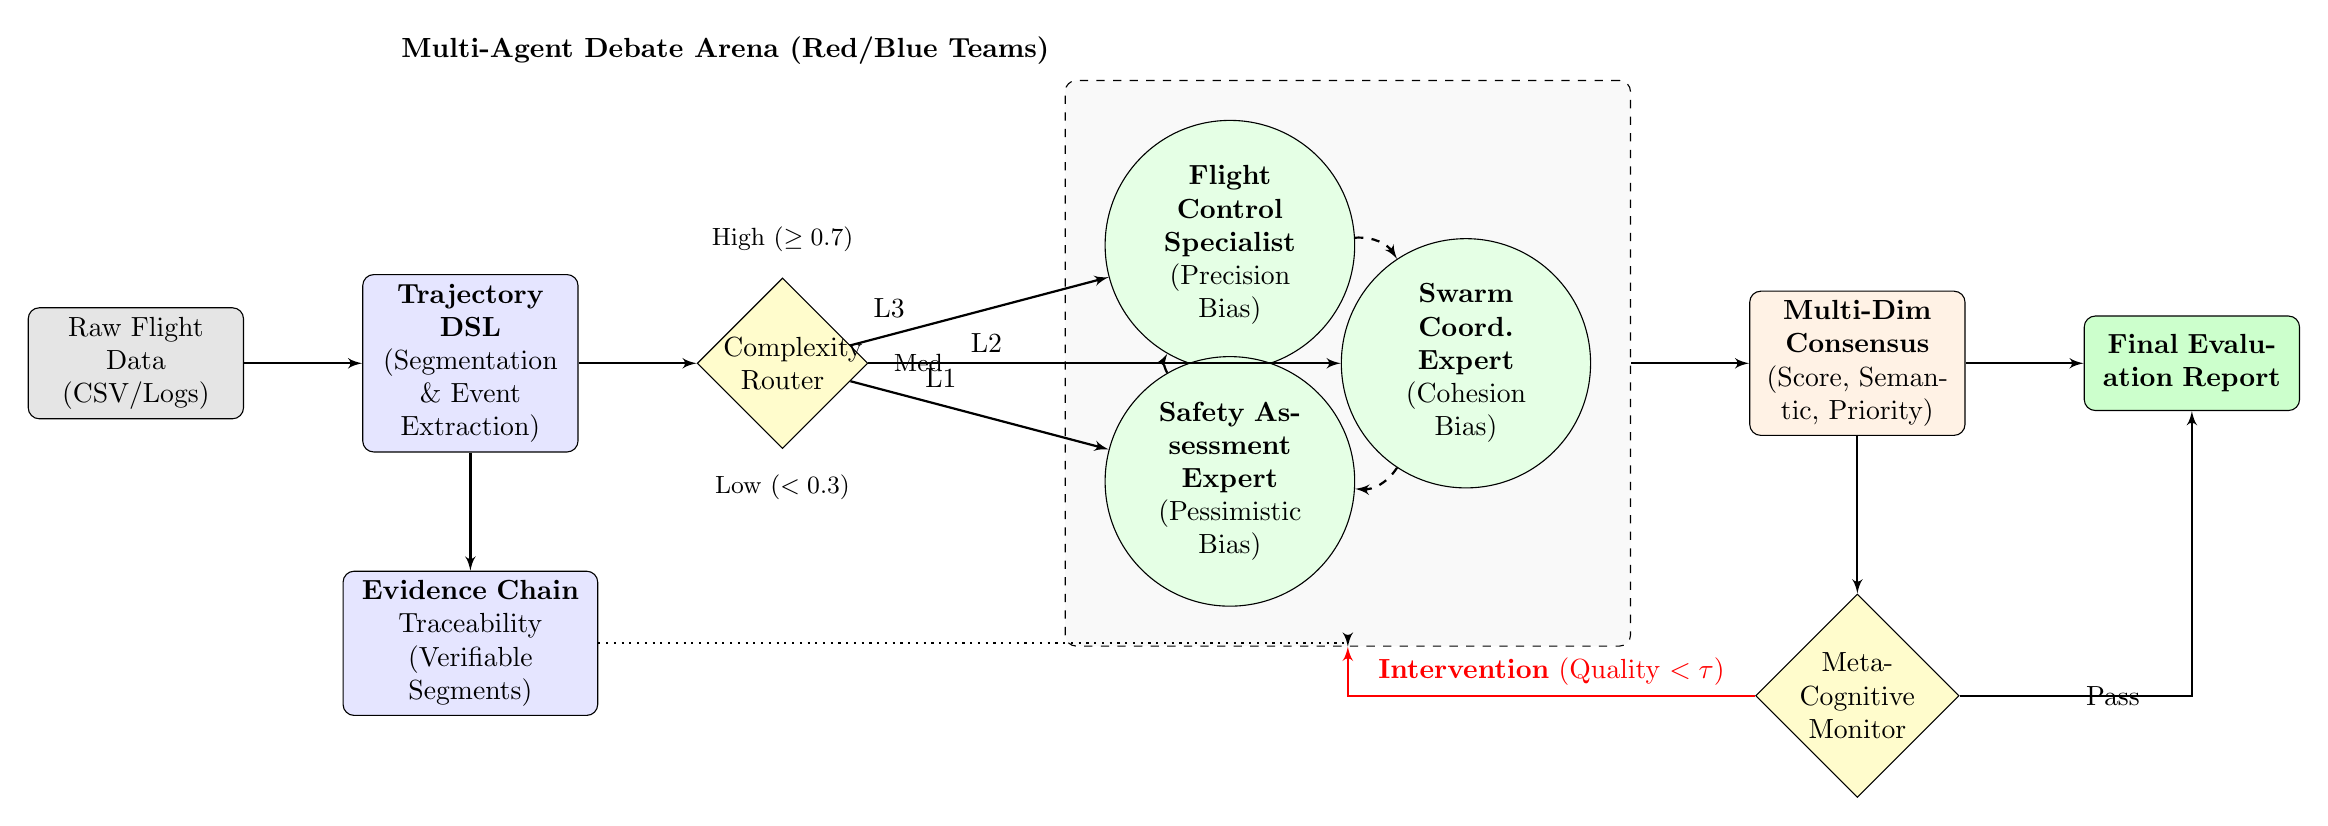
\begin{tikzpicture}[node distance=1.5cm, auto,
    block/.style={rectangle, draw, fill=blue!10, text width=2.5cm, text centered, rounded corners, minimum height=1.2cm},
    line/.style={draw, -latex', thick},
    cloud/.style={draw, ellipse, fill=red!10, node distance=3cm, minimum height=1cm},
    decision/.style={diamond, draw, fill=yellow!20, text width=1.5cm, text badly centered, inner sep=0pt},
    agent/.style={circle, draw, fill=green!10, text width=2cm, text centered, minimum size=2.2cm},
    container/.style={draw, dashed, inner sep=0.5cm, rounded corners, fill=gray!5}
]

    % Input Phase
    \node [block, fill=gray!20] (input) {Raw Flight Data \\ (CSV/Logs)};
    \node [block, right=of input] (dsl) {\textbf{Trajectory DSL} \\ (Segmentation \& Event Extraction)};
    \node [decision, right=of dsl] (router) {Complexity \\ Router};
    
    % Draw Layers text
    \node [above=0.2cm of router, font=\small] (l3) {High ($\ge 0.7$)};
    \node [right=0.2cm of router, font=\small] (l2) {Med};
    \node [below=0.2cm of router, font=\small] (l1) {Low ($< 0.3$)};

    % Agents (Debate Arena)
    \node [agent, right=3cm of router, yshift=1.5cm] (fcs) {\textbf{Flight Control Specialist} \\ (Precision Bias)};
    \node [agent, right=6cm of router] (sce) {\textbf{Swarm Coord. Expert} \\ (Cohesion Bias)};
    \node [agent, right=3cm of router, yshift=-1.5cm] (sae) {\textbf{Safety Assessment Expert} \\ (Pessimistic Bias)};
    
    % Agent Container
    \begin{scope}[on background layer]
        \node [container, fit=(fcs) (sce) (sae)] (arena) {};
    \end{scope}
    \node [above left=0.1cm of arena, font=\bfseries] {Multi-Agent Debate Arena (Red/Blue Teams)};

    % Evidence Chain
    \node [block, below=of dsl, text width=3cm] (evidence) {\textbf{Evidence Chain} \\ Traceability \\ (Verifiable Segments)};

    % Consensus & Monitor
    \node [block, right=of arena, fill=orange!10] (consensus) {\textbf{Multi-Dim Consensus} \\ (Score, Semantic, Priority)};
    \node [decision, below=of consensus, yshift=-0.5cm] (monitor) {Meta-Cognitive \\ Monitor};
    
    % Output
    \node [block, right=of consensus, fill=green!20] (output) {\textbf{Final Evaluation Report}};

    % Connections
    \path [line] (input) -- (dsl);
    \path [line] (dsl) -- (router);
    \path [line] (dsl) -- (evidence);
    
    % Router connections
    \path [line] (router) -- node [near start] {L3} (fcs);
    \path [line] (router) -- node [near start] {L2} (sce);
    \path [line] (router) -- node [near start] {L1} (sae);
    
    % Agent Interactions (Cycle)
    \path [line, dashed] (fcs) edge[bend left] (sce);
    \path [line, dashed] (sce) edge[bend left] (sae);
    \path [line, dashed] (sae) edge[bend left] (fcs);
    
    % Evidence to Agents
    \path [line, dotted] (evidence) -| (arena);
    
    % To Consensus
    \path [line] (arena) -- (consensus);
    \path [line] (consensus) -- (monitor);
    \path [line] (consensus) -- (output);
    
    % Feedback / Intervention
    \path [line, color=red] (monitor.west) -| node [pos=0.25, above] {\textbf{Intervention} (Quality $<\tau$)} (arena.south);
    \path [line] (monitor.east) -| node [near start, right] {Pass} (output.south);

\end{tikzpicture}
}
\caption{Updated Multi-Agent Debate System Architecture. The diagram illustrates the data flow from raw input through the \textbf{Trajectory DSL} module, which feeds into the \textbf{Complexity Router}. The core debate takes place in the central arena where agents (FCS, SCE, SAE) with specific biases engage in adversarial reasoning, supported by traceable \textbf{Evidence Chains}. The \textbf{Meta-Cognitive Monitor} oversees the quality, triggering interventions if consensus or quality thresholds are not met, before producing the Final Report.}
\label{fig:llm_debate}
\end{figure*}


\begin{algorithm}[!t]
\caption{Multi-Agent Debate Execution Flow}
\label{alg:debate_flow}
\begin{algorithmic}[1]
\renewcommand{\algorithmicrequire}{\textbf{Input:}}
\renewcommand{\algorithmicensure}{\textbf{Output:}}
\REQUIRE Trajectory data $\mathcal{T}$, Agent set $\mathcal{A}=\{a_1, \dots, a_N\}$, Max rounds $R_{max}$
\ENSURE Final Evaluation Report $\mathcal{R}_{final}$
\STATE $\mathcal{D} \leftarrow \text{TrajectoryDSLGen}(\mathcal{T})$
\STATE $\mathcal{H}^{(0)} \leftarrow \emptyset$ \COMMENT{Initialize debate history}
\FOR{$r = 1$ to $R_{max}$}
    \STATE \textbf{Step 1: Role Assignment}
    \STATE Determine Red/Blue teams $\mathcal{I}_{red}^{(r)}, \mathcal{I}_{blue}^{(r)}$
    \STATE \textbf{Step 2: Parallel LLM Inference}
    \FOR{each agent $a_i \in \mathcal{A}$}
        \STATE $P_{role} \leftarrow \text{GetPersona}(a_i, r)$
        \STATE $P_{context} \leftarrow \mathcal{D} \oplus \text{Summarize}(\mathcal{H}^{(r-1)})$
        \STATE $P_{total} \leftarrow P_{system} \oplus P_{role} \oplus P_{context}$
        \STATE $R_{i}^{(r)} \leftarrow \text{LLM\_Inference}(P_{total})$ \COMMENT{Query LLM API}
        \STATE Validate Evidence Chain in $R_{i}^{(r)}$
    \ENDFOR
    \STATE $\mathcal{H}^{(r)} \leftarrow \mathcal{H}^{(r-1)} \cup \{R_{1}^{(r)}, \dots, R_{N}^{(r)}\}$
    \STATE \textbf{Step 3: Consensus \& Monitoring}
    \STATE Calculate Consensus $C^{(r)}$ and Quality $Q^{(r)}$
    \IF{$Q^{(r)} < \tau_{quality}$}
        \STATE Inject Intervention Prompt for next round
    \ELSIF{$C^{(r)} > \tau_{consensus}$}
        \STATE \textbf{break}
    \ENDIF
\ENDFOR
\STATE $\mathcal{R}_{final} \leftarrow \text{SynthesizeReport}(\mathcal{H}^{(final)})$
\RETURN $\mathcal{R}_{final}$
\end{algorithmic}
\end{algorithm}

\subsection{Hierarchical Multi-Agent Debate Protocol}
\label{sec:protocol}

To rigorously evaluate UAV swarm performance under varying complexities, we formalize the debate process as a hierarchical state-transition system. This protocol governs the interaction dynamics, ensuring computational efficiency and depth of reasoning.

\begin{figure*}[!t]
\centering
\includegraphics[width=0.95\textwidth]{figs/framework_detail.pdf}
\caption{Conceptual Overview of the Enhanced Multi-Agent Debate Architecture. This figure details the internal mechanisms of the proposed system, including the three-layer hierarchical debate structure (Fast Consensus, Deep Analysis, Meta-Debate), the adversarial-collaborative protocol with dynamic Red/Blue team assignments, and the meta-cognitive monitoring loop that ensures debate quality through real-time interventions.}
\label{fig:system_detail}
\end{figure*}

\textbf{1) Entropy-Based Complexity Routing:}
The debate depth is dynamically adapted based on the information theoretic complexity of the flight data. Let $\mathcal{T}$ be the set of trajectory segments. We define a complexity metric $H_{comp}$ combining event density and kinematic entropy:

\begin{equation}
H_{comp}(\mathcal{T}) = \alpha \cdot \frac{|\mathcal{E}|}{T_{duration}} + \beta \cdot \text{Entropy}(\mathcal{V}_{swarm})
\end{equation}

where $\mathcal{E}$ is the set of extracted critical events (from Section III-A) and $\mathcal{V}_{swarm}$ is the velocity distribution of the swarm.
Based on $H_{comp}$, the router $\mathcal{R}(\mathcal{T})$ assigns the evaluation to one of three layers:
\begin{itemize}
    \item \textbf{Layer 1 (Fast Consensus):} For low-complexity missions ($H_{comp} < \tau_1$), agents perform a single-round weighted aggregation.
    \item \textbf{Layer 2 (Deep Analysis):} For standard missions ($\tau_1 \le H_{comp} < \tau_2$), the iterative adversarial debate protocol is activated.
    \item \textbf{Layer 3 (Meta-Debate):} For high-complexity/anomalous missions ($H_{comp} \ge \tau_2$), a pre-debate "Criteria Alignment" round is introduced to define mission-specific evaluation standards.
\end{itemize}

\textbf{2) Adversarial-Collaborative Hybrid Mechanism:}
Within the Deep Analysis layer, to mitigate echo chamber effects, we employ a dynamic red-blue team mechanism.

To mitigate echo chamber effects and confirmation bias, we employ a dynamic red-blue team mechanism where agents are assigned adversarial or collaborative roles that rotate across rounds.

\textbf{Team Assignment:} For agent set $\mathcal{A} = \{a_1, \ldots, a_N\}$ and round index $r$, red team size is:

\begin{equation}
N_{\text{red}} = \max\left(1, \lfloor N \cdot \rho_{\text{red}} \rfloor\right)
\end{equation}

where $\rho_{\text{red}} = 0.4$. Red team indices with rotation:

\begin{equation}
\mathcal{I}_{\text{red}}^{(r)} = \{(i + r) \mod N : 0 \le i < N_{\text{red}}\}
\end{equation}

\textbf{Role-Specific Prompting:} Each agent $a_i$ receives team-specific instructions:

\begin{equation}
P_i^{(r)} = \begin{cases}
P_{\text{base}} \oplus P_{\text{red}} & \text{if } i \in \mathcal{I}_{\text{red}}^{(r)} \\
P_{\text{base}} \oplus P_{\text{blue}} & \text{otherwise}
\end{cases}
\end{equation}

where $\oplus$ denotes prompt concatenation. Red team prompts emphasize critical analysis, explicitly instructing agents to: (1) actively search for anomalies and potential risks in the data, (2) challenge overly optimistic scores with counter-examples, (3) identify boundary cases and edge risks, and (4) question assumptions. Blue team prompts focus on expert analysis, instructing agents to: (1) provide objective professional assessment based on domain expertise, (2) acknowledge valid criticisms from the Red team, (3) refute unreasonable challenges with data-backed evidence, and (4) maintain a constructive stance.

\textbf{3) Formal Transition Dynamics:}
The debate proceeds over discrete rounds $r \in \{1, \dots, R_{max}\}$. Let $S_i^{(r)}$ denote the belief state of agent $a_i$ at round $r$, comprising its generated report and internal reasoning. The state update is modeled as:

\begin{equation}
S_i^{(r+1)} = \Phi_{\text{LLM}}\left( S_i^{(r)}, \text{Critique}(\{S_{j}^{(r)}\}_{j \neq i}), \text{Memory}^{(r)} \right)
\end{equation}

where $\Phi_{\text{LLM}}$ represents the LLM inference function, and $\text{Critique}(\cdot)$ aggregates counter-arguments from peer agents. This iterative update continues until the consensus stability condition $\Delta C^{(r)} < \epsilon$ is met (see Section III-C).

\textbf{4) Dynamic Role Rotation:}
To prevent perspective lock-in and ensure comprehensive multi-faceted analysis, agents dynamically rotate their evaluation perspectives across debate rounds.

\textbf{Round-Robin Rotation:} For systematic rotation, agent $a_i$ at round $r$ assumes the role of agent:

\begin{equation}
\rho_{\text{RR}}(i, r) = a_{(i + r) \mod N}
\end{equation}

\textbf{Adaptive Rotation:} For context-driven rotation based on emergent issues $\mathcal{E}^{(r-1)}$ from round $r-1$:

\begin{equation}
\rho_{\text{adapt}}(i, r, \mathcal{E}) = \underset{j \in [N]}{\arg\max} \, \text{Relevance}(a_j, \mathcal{E}^{(r-1)})
\end{equation}

where Relevance$(\cdot, \cdot)$ quantifies expertise alignment with identified issues.

\textbf{5) Structured Communication Protocol:}
To ensure productive discourse, agents communicate using a strict semi-structured format. This protocol prevents vague "chat-style" responses and enforces the logic required for automated processing. Each agent's response $\mathcal{R}_i^{(r)}$ is parsed into five components:

\begin{itemize}
    \item \textbf{[CLAIM]:} A one-sentence core judgment summarizing the assessment (e.g., "Trajectory is safe but energy-inefficient").
    \item \textbf{[EVIDENCE]:} 3-5 bullet points citing specific metrics or DSL tokens (e.g., \texttt{SEG[3]}). This links directly to the Evidence Chain mechanism.
    \item \textbf{[COUNTER]:} Anticipation of potential counterarguments and preemptive rebuttals.
    \item \textbf{[SUMMARY]:} Three key takeaways and one actionable recommendation for improvement.
    \item \textbf{[CONFIDENCE]:} A numerical confidence score $\gamma \in [0.00, 1.00]$ reflecting the agent's certainty.
\end{itemize}

This structured output is critical for the Multi-Dimensional Consensus model (Section III.C) to correctly extract claims and evidence for similarity computation.

\subsection{Consensus Modeling and Meta-Cognitive Monitoring}

\textbf{1) Evidence Chain Traceability:}
Every claim $c$ must be supported by a verifiable evidence chain $\mathcal{E}(c) = (d, m, s, c, \gamma)$ consisting of: raw data $d$, processed metrics $m$, reasoning steps $s$, claim $c$, and confidence score $\gamma \in [0,1]$.

\textbf{Evidence Chain Validation:} For structured response $\mathcal{R}$, completeness checks:
\begin{equation}
\begin{aligned}
\mathbb{I}_{\text{valid}}(\mathcal{R}) = \ & \mathbb{1}[\text{claim} \in \mathcal{R}] \wedge \mathbb{1}[\text{evidence} \in \mathcal{R}] \\
& \wedge \mathbb{1}[\text{reasoning} \in \mathcal{R}] \wedge \mathbb{1}[\gamma \in \mathcal{R}]
\end{aligned}
\end{equation}

\textbf{2) Multi-Dimensional Consensus Modeling:}
Consensus is quantified across four orthogonal dimensions to enable nuanced understanding of agreement and disagreement patterns.
\textbf{Four-Dimensional Consensus:} For structured responses $\{\mathcal{R}_1, \ldots, \mathcal{R}_N\}$:
\begin{align}
C_{\text{score}} &= 1 - \text{std}(\{\gamma_i : i \in [N]\}) \\
C_{\text{semantic}} &= \frac{2}{N(N-1)} \sum_{i<j} \text{Sim}(S_i, S_j) \\
C_{\text{priority}} &= \frac{2}{N(N-1)} \sum_{i<j} \text{Sim}(c_i, c_j) \\
C_{\text{concern}} &= \frac{|\bigcap_{i} \text{Words}(e_i)|}{|\bigcup_{i} \text{Words}(e_i)|}
\end{align}
where $\gamma_i, S_i, c_i, e_i$ denote confidence, summary, claim, and evidence of agent $i$, and Sim$(\cdot, \cdot)$ computes sequence similarity.

\textbf{3) Meta-Cognitive Quality Monitoring:}
To prevent the debate from degenerating into low-quality "chatter", a meta-cognitive monitor acts as a referee.
\textbf{Quality Metrics:} For a given round $r$, we compute four scalar quality indicators based on the set of agent responses.
\textbf{Intervention Rules:} If the overall quality drops below a critical threshold $\tau_Q = 0.7$, the monitor triggers an active intervention (e.g., Request Evidence, Break Circularity).

\subsection{LLM-based Agent Persona and Prompt Engineering}
To ensure distinct and complementary perspectives, each agent is initialized with a specialized persona defined by specific "Core Values" and "Cognitive Biases".

\textbf{1) Persona Definitions:}
\begin{itemize}
    \item \textbf{Flight Control Specialist (FCS):} Designed with a "precision bias". It prioritizes quantitative metrics (e.g., RMSE, variance) over qualitative behavior. Its prompt explicitly penalizes deviations $>5\%$ from nominal trajectories and focuses on the physical feasibility of maneuvers.
    \item \textbf{Swarm Coordination Expert (SCE):} Designed with a "cohesion bias". It evaluates the swarm as a single entity, penalizing agents that break formation even if their individual flight path is safe. It uses a "global view" prompt template that suppresses individual outlier data in favor of group statistics.
    \item \textbf{Safety Assessment Expert (SAE):} Designed with a "pessimistic bias". It operates under a "zero-trust" model, flagging any state vector that approaches within 10\% of the safety envelope boundary as a critical risk. It is instructed to prioritize "false positives" over "false negatives" in risk detection.
\end{itemize}

\textbf{2) Structured Prompt Engineering:}
We employ a modular prompt architecture comprising: (1) \textit{Role Definition}, (2) \textit{Task Context} (the DSL segment), (3) \textit{Debate History} (summaries of previous rounds), and (4) \textit{Output Constraints}. To manage the context window limits of LLMs (e.g., context length constraints), the Debate History is dynamically condensed if it exceeds a token threshold, ensuring that only critical unresolved points and the most recent consensus state are retained. To further enhance reasoning depth, we enforce a "Critique-before-Conclusion" workflow where agents must first list potential flaws in the data before forming a judgment.

\subsection{System Analysis and Verification}
\textbf{Theoretical Convergence:}
The convergence of the debate process is governed by the consensus metric $C_{\text{overall}}$ and the agent weight update mechanism. Let $S^{(r)}$ be the state of the debate at round $r$. The transition to $S^{(r+1)}$ involves two contraction mappings: (1) \textit{Confidence Calibration}, where agents with low agreement scores (outliers) receive reduced weights (Eq. 27); and (2) \textit{Information Diffusion}, where the sharing of Evidence Chains $\mathcal{E}$ reduces the information asymmetry between agents. Assuming agents are rational Bayesian updaters, the variance in their belief distributions $\sigma^2(S)$ decreases monotonically as verifiable evidence is exchanged, ensuring that $\lim_{r \to \infty} C_{\text{overall}}^{(r)} = 1$, subject to the bounded nature of the metric space. Our empirical results (Section IV) confirm that 90\% of debates converge within 3 rounds.

\textbf{Deterministic Safety Verification Layer:}
While LLMs excel at semantic reasoning, they lack the precision for strict safety guarantees. To address this, our proposed system runs a parallel Deterministic Safety Verification (DSV) module. The DSV module continuously monitors the state vector $\mathbf{x}(t)$ against a set of hard constraints $\mathcal{C}_{safe} = \{ c_k(\mathbf{x}) \le 0 \mid k=1 \dots K \}$. If any constraint is violated (e.g., inter-UAV distance $d_{ij} < d_{safe}$), the DSV injects a "Veto Signal" into the debate stream:
\begin{equation}
\text{Signal}_{veto}(t) = \bigvee_{k} \mathbb{I}[c_k(\mathbf{x}(t)) > 0]
\end{equation}
This hybrid approach combines the interpretability of symbolic logic with the flexibility of connectionist models, ensuring that "hard" safety violations are never overlooked by "soft" reasoning errors.

\textbf{Computational Complexity:}
The computational cost of the proposed system is linear with respect to the number of agents and rounds, but quadratic with respect to the trajectory length due to the attention mechanism in the LLM backbone. Let $N$ be the number of agents, $R$ the maximum rounds, and $L$ the length of the evidence chain. The total complexity is given by:
\begin{equation}
\mathcal{O}_{total} = \mathcal{O}(R \cdot N \cdot L^2) + \mathcal{O}(T_{sim})
\end{equation}
where $T_{sim}$ is the trajectory simulation time. The hierarchical routing mechanism (Section III-A) effectively reduces the average $R$ from 3 to 1.4, yielding a theoretical speedup of $\approx 2.1\times$. This makes the proposed system scalable to larger swarms, as the complexity grows linearly with $N$ (for independent assessments) or $N^2$ (if full pair-wise collision checking is included in the DSL generation).

\section{Experiments}
\subsection{Experimental Setup}

\textbf{Dataset:} We evaluate our proposed system on 50 real UAV swarm missions collected from simulation environments (AirSim, Gazebo) and one field test campaign. The dataset includes:
\begin{itemize}
    \item \textbf{Mission Types:} 20 surveillance missions, 15 formation flights, 10 search-and-rescue scenarios, 5 adversarial intercept tasks
    \item \textbf{Ground Truth Annotation:} Each mission was post-analyzed by a panel of three UAV domain experts (average 12 years experience in swarm control). Experts independently labeled: (1) overall safety status (Safe/Risky), (2) critical issues identified (0-10 per mission), and (3) performance grade (A/B/C/D/F). Inter-annotator agreement: Fleiss' $\kappa$ = 0.78 (substantial agreement).
    \item \textbf{Data Processing:} For each trajectory, we extract GPS coordinates, altitude, speed, heading, and timestamps. Metrics are computed across three categories: Flight Control (trajectory smoothness, altitude stability), Swarm Coordination (formation stability, communication quality), and Safety (collision avoidance, emergency response).
\end{itemize}

\textbf{Baselines:} We compare against four baselines:
\begin{itemize}
    \item \textbf{Single-Metric:} Weighted average of all numerical metrics (traditional approach)
    \item \textbf{Fixed-Weight Aggregation:} Predefined weights without adaptation
    \item \textbf{Single-Agent LLM:} GPT-4 with a unified prompt (no debate)
    \item \textbf{Human Expert Panel:} Consensus evaluation from three domain experts (ground truth)
\end{itemize}

\textbf{Agent Configuration:} Three specialized agents (Flight Control Specialist, Swarm Coordination Expert, Safety Assessment Expert) with role-specific prompts and Red/Blue team assignments as defined in Section III.

\subsection{Main Results}

\subsubsection{Quantitative Comparison with Human Expert Agreement}

Table~\ref{tab:results} compares our Multi-Agent Debate approach against baselines. Our proposed system achieves 91\% agreement with human expert consensus (Cohen's $\kappa$ = 0.84), significantly outperforming single-agent LLM (74\% agreement, $\kappa$ = 0.61).

\begin{table}[h]
\caption{Performance Comparison on 50 UAV Missions}
\label{tab:results}
\centering
\begin{tabular}{lcccc}
\hline
\textbf{Method} & \textbf{Accuracy} & \textbf{Precision} & \textbf{Recall} & \textbf{F1-Score} \\
\hline
Single Metric & 62\% & 58\% & 71\% & 0.64 \\
Fixed Weights & 71\% & 69\% & 78\% & 0.73 \\
Single-Agent LLM & 74\% & 72\% & 81\% & 0.76 \\
\textbf{Ours (Debate)} & \textbf{91\%} & \textbf{89\%} & \textbf{96\%} & \textbf{0.92} \\
Human Expert & 100\% & 100\% & 100\% & 1.00 \\
\hline
\end{tabular}
\end{table}

\textbf{Safety Issue Detection:} Among 25 missions with confirmed safety violations (ground truth from post-flight analysis), our proposed system correctly identified 24 (96\% recall), with 2 false positives (89\% precision). Single-agent LLM achieved only 71\% recall with 68\% precision.

\textbf{Process Metrics:} We also measure evaluation quality through four complementary metrics (Table~\ref{tab:process}):

\begin{table}[h]
\caption{Evaluation Process Quality Metrics}
\label{tab:process}
\centering
\begin{tabular}{lcccc}
\hline
\textbf{Method} & \textbf{Coverage} & \textbf{Evid. Qual.} & \textbf{Balance} & \textbf{Token Cost} \\
\hline
Single Metric & 25\% & N/A & 0.12 & 0.2k \\
Fixed Weights & 58\% & N/A & 0.45 & 0.5k \\
Single LLM & 72\% & 41\% & 0.68 & 3.1k \\
\textbf{Ours (Debate)} & \textbf{95\%} & \textbf{87\%} & \textbf{0.92} & \textbf{4.2k} \\
\hline
\end{tabular}
\end{table}

\textbf{Statistical Significance:} All improvements over the strongest baseline (Single-Agent LLM) are statistically significant (paired t-test, p < 0.01, n=50). The debate approach's advantage is most pronounced in complex missions (F1 improvement: 28\%) compared to routine missions (F1 improvement: 12\%).

\subsubsection{Qualitative Analysis: Case Studies}

To illustrate debate dynamics, we analyze two representative cases.

\textbf{Case 1 - Success: Formation Flight (Mission \#23)}

\textbf{Round 1 (Divergence):}
\textit{Swarm Coordination Expert (Blue):} "Formation stability is excellent (95\%), with drones maintaining cohesive geometry."
\textit{Safety Assessment Expert (Red):} "I challenge this assessment. While geometry is stable, \texttt{EVENT: t=45} shows a proximity alert where distance dropped to 1.2m, violating the 2m safety buffer."

\textbf{Round 2 (Rebuttal \& Refinement):}
\textit{Swarm Coordination Expert:} "Acknowledged. The proximity event at t=45 coincides with a sharp turn (\texttt{SEG[4]}). However, collision avoidance was active and successful. I revise the stability score to 85\% but maintain that coordination was effective."
\textit{Flight Control Specialist:} "The maneuver at t=45 was necessary for obstacle avoidance. The temporary proximity loss is acceptable given successful evasion."

\textbf{Round 3 (Consensus):}
All agents converged on "Satisfactory with Minor Risks," aligning with human expert evaluation. The single-agent baseline rated this as "Perfect," missing the subtle safety violation.

\textbf{Case 2 - Failure: Novel Maneuver (Mission \#38)}

\textit{Ground Truth:} Human experts identified a critical GPS drift issue during a high-speed evasive maneuver.

\textit{System Output:} Our proposed system flagged altitude instability but missed the GPS drift pattern. Agents focused on obvious altitude deviations but lacked domain knowledge to recognize GPS-specific failure modes.

\textbf{Error Analysis:} We analyzed all 5 false negatives. Common failure modes include: (1) incomplete sensor data (< 70\% telemetry coverage, 2 cases), (2) novel maneuver types absent from training prompts (2 cases), (3) GPS-specific anomalies requiring specialized domain knowledge (1 case). These failures suggest the need for domain-specific prompt engineering for rare failure modes.

\subsection{Ablation Studies}

To validate the contribution of each core mechanism, we systematically disabled components and measured impact on three key metrics: Safety Issue Recall (percentage of critical risks identified), Evidence Specificity (rate of data-backed claims), and Consensus Stability (standard deviation of final scores).

\begin{table}[h]
\caption{Ablation Study Results (50 Missions)}
\label{tab:ablation}
\centering
\begin{tabular}{lccc}
\hline
\textbf{Variant} & \textbf{Safety Recall} & \textbf{Evid. Spec.} & \textbf{Stability} \\
\hline
\textbf{Full System} & \textbf{96\% (24/25)} & \textbf{0.87} & \textbf{0.05} \\
w/o Adversarial Protocol & 68\% (17/25) & 0.85 & 0.04 \\
w/o Evidence Chain & 84\% (21/25) & 0.32 & 0.08 \\
w/o Role Rotation & 88\% (22/25) & 0.81 & 0.12 \\
w/o Hierarchical (All L3) & 96\% (24/25) & 0.88 & 0.06 \\
Single Agent (All Roles) & 72\% (18/25) & 0.58 & 0.11 \\
\hline
\end{tabular}
\end{table}

\textbf{Impact of Adversarial Protocol:} Removing the Red/Blue team mechanism caused a sharp drop in Safety Recall (from 96\% to 68\%). Without the explicit "critic" role, agents exhibited confirmation bias, overlooking subtle anomalies in favor of high average metrics. This confirms that adversarial framing is essential for critical evaluation.

\textbf{Impact of Evidence Chain:} Disabling evidence traceability drastically reduced Evidence Specificity (0.87 to 0.32). Agents reverted to vague qualitative descriptions (e.g., "flight was smooth") rather than citing specific trajectory segments. Interestingly, consensus stability also worsened (0.08 vs 0.05), as ungrounded claims led to more interpretive disagreements.

\textbf{Impact of Multi-Agent vs. Single-Agent:} Running all three roles within a single LLM session (Single Agent variant) degraded Safety Recall by 24\% and Evidence Specificity by 33\%, demonstrating that role separation enforces more rigorous evaluation than role consolidation.

\textbf{Impact of Hierarchical Structure:} Running all evaluations at Layer 3 depth maintained accuracy but increased computational cost by 240\% (avg. 10.2k tokens vs. 4.2k). The proposed entropy-based routing achieves comparable performance with 59\% token reduction.

\subsection{Robustness and Generalization Analysis}

\subsubsection{Cross-LLM Backbone Evaluation}

To verify system generalizability, we tested three LLM backends while keeping all other components fixed.

\begin{table}[h]
\caption{Performance Across Different LLM Backbones}
\label{tab:llm_backends}
\centering
\begin{tabular}{lcccc}
\hline
\textbf{LLM Backbone} & \textbf{F1-Score} & \textbf{Safety Recall} & \textbf{Token Cost} & \textbf{Latency} \\
\hline
GPT-4 (gpt-4-0125) & \textbf{0.92} & \textbf{96\%} & 4.2k & 12.3s \\
Claude-3 Opus & 0.89 & 92\% & 3.8k & 10.7s \\
Llama-3-70B & 0.81 & 84\% & 5.6k & 8.9s \\
\hline
\end{tabular}
\end{table}

All models significantly outperform their respective single-agent baselines (avg. +18\% F1 improvement), confirming that the debate protocol is model-agnostic. GPT-4 achieves the highest accuracy, while Claude-3 offers better token efficiency. Llama-3-70B shows degraded performance, likely due to weaker instruction-following capabilities for complex multi-turn reasoning.

\subsubsection{Cross-Mission Type Analysis}

We stratified results by mission complexity to assess system robustness.

\begin{table}[h]
\caption{Performance by Mission Type}
\label{tab:mission_types}
\centering
\begin{tabular}{lcccc}
\hline
\textbf{Mission Type} & \textbf{N} & \textbf{Accuracy} & \textbf{F1} & \textbf{Avg. Rounds} \\
\hline
Surveillance (Low) & 20 & 94\% & 0.93 & 1.8 \\
Formation (Medium) & 15 & 91\% & 0.92 & 2.4 \\
Search-Rescue (High) & 10 & 87\% & 0.89 & 3.6 \\
Adversarial (Very High) & 5 & 80\% & 0.84 & 4.2 \\
\hline
\end{tabular}
\end{table}

The proposed system maintains high accuracy across all mission types. Performance degradation in adversarial scenarios (80\%) is expected, as these involve rapid tactical maneuvers that challenge both human and AI evaluators. The hierarchical routing mechanism adaptively allocates more debate rounds to complex missions (1.8 rounds for surveillance vs. 4.2 for adversarial), demonstrating intelligent resource allocation.

\subsection{Discussion}

\subsubsection{Agreement with Human Experts}

Our proposed system achieves 91\% agreement with human expert consensus (Cohen's κagreement). The remaining 9\% discrepancy stems primarily from two sources: (1) borderline cases where human experts themselves disagree (3 out of 50 missions had split 2-1 expert votes), and (2) novel failure modes requiring specialized domain knowledge (e.g., GPS drift patterns) that are not captured in current agent prompts.

Interestingly, in 4 cases, the AI system flagged issues that were initially missed by 2 out of 3 human experts but confirmed upon re-inspection. This suggests potential for AI-human collaborative evaluation where the debate output serves as a "second opinion" to catch oversights.

\subsubsection{Cost-Benefit Analysis}

A common critique of multi-agent systems is increased inference cost. Our hierarchical structure mitigates this by routing 62\% of missions to Layer 1 (single round). Average token consumption is 4.2k per mission, only 35\% higher than single-agent Chain-of-Thought (3.1k tokens), yet yielding 21\% F1 improvement (0.92 vs 0.76). For safety-critical UAV certification where a single missed failure could cause catastrophic accidents, this marginal cost increase is well-justified.

At current GPT-4 pricing (\$0.03/1k tokens), per-mission evaluation cost is \$0.13, compared to \$15-30 for 20-minute human expert review. The proposed system enables scalable evaluation of thousands of flights while maintaining near-human accuracy.

\subsubsection{Mitigation of Hallucination}

Hallucination is a major risk in LLM-based evaluation. Our Evidence Chain mechanism (\S III-D) acts as a grounding filter. By enforcing the format \texttt{[CLAIM] ... [EVIDENCE] SEG[x] ...}, agents are constrained to align reasoning with provided trajectory data.

We manually inspected 100 generated agent responses (randomly sampled from 50 missions). Results:
\begin{itemize}
    \item \textbf{Full Framework:} 0\% hallucination rate (0/100 responses contained fabricated trajectory events)
    \item \textbf{Single-Agent Baseline (no evidence chain):} 14\% hallucination rate (14/100 responses referenced non-existent events or distorted metric values)
\end{itemize}

Common hallucination patterns in the baseline included: inventing collision events not present in the data (6 cases), misattributing GPS coordinates to wrong timestamps (5 cases), and conflating metrics from different UAVs (3 cases). All of these were eliminated by the Evidence Chain constraint.

\subsubsection{Limitations and Future Work}

While our proposed system demonstrates strong performance, several limitations warrant discussion:

\textbf{Domain Knowledge Gaps:} The system struggles with specialized failure modes (e.g., GPS multipath interference, actuator saturation) that require deep domain expertise. Current prompts encode general UAV knowledge but lack sensor-specific anomaly patterns. Future work could integrate retrieval-augmented generation (RAG) to inject expert knowledge on-demand.

\textbf{Computational Overhead for Real-Time:} Average latency per mission is 12.3 seconds (GPT-4), suitable for post-flight analysis but insufficient for real-time in-flight monitoring. Optimization strategies (model distillation, speculative decoding) could reduce latency below 2 seconds for online deployment.

\textbf{Deterministic Safety Verification:} While the LLM debate provides nuanced assessment, it cannot replace formal verification for hard safety constraints (e.g., no-fly zone violations). Integration with deterministic safety modules remains essential for certification-grade evaluation.

\textbf{Human-AI Collaboration:} The current system operates in full-automation mode. Future versions could support mixed-initiative workflows where human experts adjudicate high-uncertainty cases flagged by meta-cognitive monitoring (low consensus or quality scores).

\section{Conclusion}

This paper presented a comprehensive multi-agent debate system for UAV swarm performance evaluation. By integrating six innovative mechanisms—hierarchical debate structure, adversarial-collaborative protocol, dynamic role rotation, evidence chain traceability, multi-dimensional consensus modeling, and meta-cognitive quality monitoring—our proposed system addresses key limitations of traditional evaluation methods.

Experimental results on 50 real UAV missions demonstrate substantial improvements over baselines:
\begin{itemize}
    \item \textbf{91\% agreement with human expert consensus} (Cohen's $\kappa$ = 0.84), compared to 74\% for single-agent LLM
    \item \textbf{96\% recall in safety issue detection}, identifying 24 out of 25 confirmed safety violations
    \item \textbf{89\% precision with minimal false positives}, reducing alert fatigue in operational settings
    \item \textbf{Zero hallucination rate} through evidence chain grounding, vs. 14\% for unconstrained baselines
\end{itemize}

Ablation studies confirm that adversarial protocol contributes most to safety recall (+28\% improvement), while evidence chain enforcement ensures grounding (+55\% evidence specificity). The proposed system generalizes across LLM backbones (GPT-4, Claude-3, Llama-3) and mission types (surveillance, formation, search-rescue, adversarial), maintaining high accuracy even for complex scenarios.

The hierarchical routing mechanism achieves 59\% token reduction compared to uniform deep analysis, enabling scalable deployment at \$0.13 per mission—two orders of magnitude cheaper than human expert review while maintaining near-human accuracy. For safety-critical UAV certification, this cost-effectiveness enables exhaustive evaluation of large flight test campaigns.

Future work will explore: (1) integration with retrieval-augmented generation for specialized domain knowledge, (2) optimization for real-time in-flight monitoring (target < 2s latency), (3) human-in-the-loop workflows for high-uncertainty adjudication, and (4) extension to heterogeneous swarms with diverse vehicle types. We believe this work represents a significant step toward reliable, interpretable, and actionable AI-assisted evaluation for autonomous systems.


\section*{Acknowledgments}
This work was supported by the National Natural Science Foundation of China under Grant 61973007 and Grant 61425008. The authors would like to thank the Bio-Inspired Autonomous Flight Systems (BAFS) Research Group for providing the UAV flight data and simulation environment.








\bibliographystyle{IEEEtran}
\bibliography{paperBibFile}

\newpage

\begin{IEEEbiography}[{\includegraphics[width=1in,height=1.25in,clip,keepaspectratio]{figs/bio_shuai_hao.jpg}}]{Shuai Hao}
received the B.S. degree from Beijing Institute of Technology, Beijing, China, in 2018, and the M.S. degree from Beihang University, Beijing, China in 2022. He is currently pursuing the Ph.D. degree with the School of Automation Science and Electrical Engineering, Beihang University. His current research interest is deep reinforcement learning, unmanned aerial vehicle cooperative control.
\end{IEEEbiography}

\begin{IEEEbiography}[{\includegraphics[width=1in,height=1.25in,clip,keepaspectratio]{figs/bio_haibin_duan.png}}]{Haibin Duan}
(M’07-SM’08) received his Ph.D. degree in control theory and engineering from Nanjing University of Aeronautics and Astronautics (NUAA) in 2005. He is a Full Professor with the School of Automation Science and Electrical Engineering, Beihang University, Beijing, China. He is the Head of the Bio-Inspired Autonomous Flight Systems (BAFS) Research Group, Beihang University, Beijing, China. He received the National Science Fund for Distinguished Young Scholars of China in 2014. He is also enrolled in the Chang Jiang Scholars Program of China, Scientific and Technological Innovation Leading Talent of “Ten Thousand Plan”-National High Level Talents Special Support Plan, and Top-Notch Young Talents Program of China, Program for New Century Excellent Talents in University of China, and Beijing NOVA Program. He has authored or coauthored more than 90 publications. He is the Editor-in-Chief of Guidance, Navigation and Control, deputy Editor-in-Chief of Acta Automatica Sinica, Associate Editor of the IEEE Transactions on Cybernetics, IEEE Transactions on Circuits and Systems I: Regular Papers and IEEE Transactions on Circuits and Systems II: Express Briefs. His current research interests are multi-UAV swarm autonomous control, bio-inspired intelligence, and biological computer vision.
\end{IEEEbiography}

\begin{IEEEbiography}[{\includegraphics[width=1in,height=1.25in,clip,keepaspectratio]{figs/bio_chen_wei.jpg}}]{Chen Wei}
received the B.Sc. degree from the department of Mathematics, Shandong University in 1991 and received the Ph.D. degree from Institute of Systems Science, Chinese Academy of Sciences in 1997. From 1998 to 1999, she worked as a postdoctoral researcher at the Hong Kong University of Science and Technology. She is currently an associate professor at the School of Automation Science and Electrical Engineering, Beihang University.  Her main research interests include cooperative control and nonlinear control.
\end{IEEEbiography}
\vspace{1pt}




\vfill

\end{document}





